\section{Coexistence Scenarios}

The previous section investigated the borders where stable cycles disappear.
We can see that parameter regions where only one stable cycle exists (``Type A'') can overlap.
For example, the upper border where the cycle $\Cycle{\A^5\B^3\C^5\D^3}$ disappears, marked blue in \Cref{fig:final.regions.E.halved}, is above the lower border where the stable cycle $\Cycle{\A^4\B^3\C^4\D^3}$ disappears, marked red.
This means that there is a coexistence of the cycles in the overlapping parameter region, marked with the point $M$.
This section will take a look at all possible coexistence scenarios of cycles starting with the simplest case, a single ``Type A'' parameter region.

\begin{figure}
    \centering
    \begin{subfigure}{0.4\textwidth}
        \centering
        \includegraphics[width=\textwidth]{60_MinimalRepr/2D_Regions_E/result.png}
        \caption{Showing $E_{16}$}
        \label{fig:final.regions.E.halved}
    \end{subfigure}
    \begin{subfigure}{0.4\textwidth}
        \centering
        \includegraphics[width=\textwidth]{60_MinimalRepr/2D_Regions_F/result.png}
        \caption{Showing $F_{16}$}
        \label{fig:final.regions.F.halved}
    \end{subfigure}
    \caption{2D Period Regions of Halved Final Model Showing a ``Type A'' and a ``Type B'' Region}
\end{figure}

\subsection{Only One ``Type A'' Parameter Region}

As mentioned above, the simplest case of coexistence in this model is the existence of a stable cycle of a ``Type A'' parameter region on its own.
A point where this is the case is the point $L$ in \Cref{fig:final.regions.E.halved}.
Here there is only one stable cycle, $\Cycle{\A^5\B^3\C^5\D^3}$.

\subsection{Two ``Type A'' Parameter Regions Overlapping}

``Type A'' parameter regions can overlap with one another.
This can happen in four different ways.
Assuming the stable cycle of the starting parameter region is $\Cycle{\A^x\B^y\C^x\D^y}$, it can overlap with parameter regions, where either one of the following cycles is stable
\begin{enumerate*}
    \item $\Cycle{\A^{x-1}\B^y\C^{x-1}\D^y}$,
    \item $\Cycle{\A^x\B^{y+1}\C^x\D^{y+1}}$,
    \item $\Cycle{\A^{x+1}\B^y\C^{x+1}\D^y}$, and
    \item $\Cycle{\A^x\B^{y-1}\C^x\D^{y-1}}$.
\end{enumerate*}
For this concrete case pictured in \Cref{fig:final.regions.E.halved}, it results in the following parameter regions
\begin{enumerate*}
    \item $\P_{\A^5\B^3\C^5\D^3, \A^4\B^3\C^4\D^3}$ marked with $M$,
    \item $\P_{\A^5\B^3\C^5\D^3, \A^5\B^4\C^5\D^4}$ marked with $N$,
    \item $\P_{\A^5\B^3\C^5\D^3, \A^6\B^3\C^6\D^3}$ marked with $O$, and
    \item $\P_{\A^5\B^3\C^5\D^3, \A^5\B^2\C^5\D^2}$ marked with $P$.
\end{enumerate*}
